\subsection{Summary of product functionality}
% Podsumowanie (przegląd) zrealizowanych funkcji finalnego produktu
% Ilustracje (screenshoty) do omawianych funkcji. Mile widziane są opis poszczególnych okien ze wskazaniem co na nich widać

In the \nameref{section:functional-requirements} section we have defined Folder's and Designer's user stories and assigned priorities to them.
All the requirements of priority 3 (high) have been realized.
Almost all the requirements of priority 2 (medium) have been resolved.
And most of the requirements of priority 1 (low) have been addressed as well.
\smallskip

In this section we have reviewed the covered functionality from the end user's perspective using screenshots of the end product.
Each section presents some part of the application and lists user stories that are addressed in a given view.
Overlaid on the screenshots are markers that describe which functionality is addressed in which part of the UI.
The format of each marker is $NX$, where $N$ is a letter - either $F$ or $D$ depicting whether  
the highlighted part of the UI corresponds to a \textbf{F}older's user story or a \textbf{D}esigner's user story.
And $X$ represents a user story's sequence number, assigned to it previously in the section \nameref{section:functional-requirements}.

\subsubsection{Guide Viewer}

Folder's user stories:
\begin{enumerate}
	\setcounter{enumi}{0}
	\requirement{3}{load an Instruction}
	\requirement{3}{view the 3D representation of the Instruction step}
	\requirement{3}{switch to the next step in the Instruction}
	\requirement{3}{switch to the previous step in the Instruction}
	\requirement{3}{see the Transition between two Instruction steps}
	\requirement{2}{pause the Transition at any time}
	\requirement{2}{rewind the Transition}
	\requirement{2}{forward the Transition}
	\requirement{3}{rotate the Model in 3D space}
	\requirement{3}{zoom the Model in and out in 3D space}
	\requirement{1}{see creases of the Model} 
	\requirement{2}{distinguish paper's top and bottom sides} 

	\setcounter{enumi}{13}

	\requirement{3}{navigate between simulator and community views} 
\end{enumerate}

\begin{figure}[H]
  	\centering
    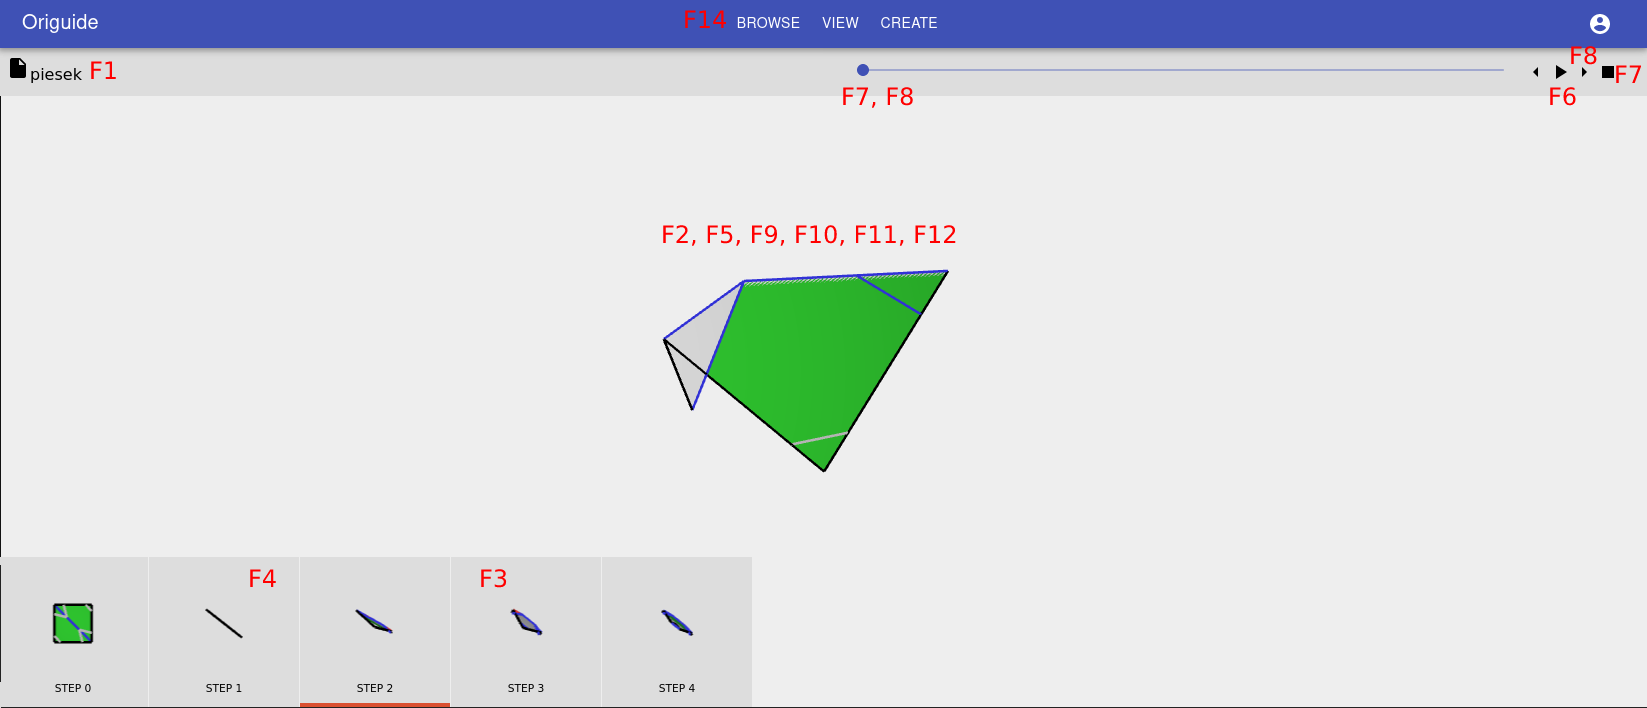
\includegraphics[width=\textwidth]{assets/5-guideViewer.png}
\end{figure}

\subsubsection{Guide Browser}

Folder's user stories:
\begin{enumerate}
	\setcounter{enumi}{14}
	\requirement{3}{view Instructions uploaded by other users} 
\end{enumerate}

Designer's user stories:
\begin{enumerate}
	\setcounter{enumi}{0}
	\requirement{3}{upload an Instruction}
	\requirement{3}{view my Instructions}
	\requirement{3}{delete my Instructions}
	\requirement{3}{update my Instructions}
\end{enumerate}

\begin{figure}[H]
  	\centering
    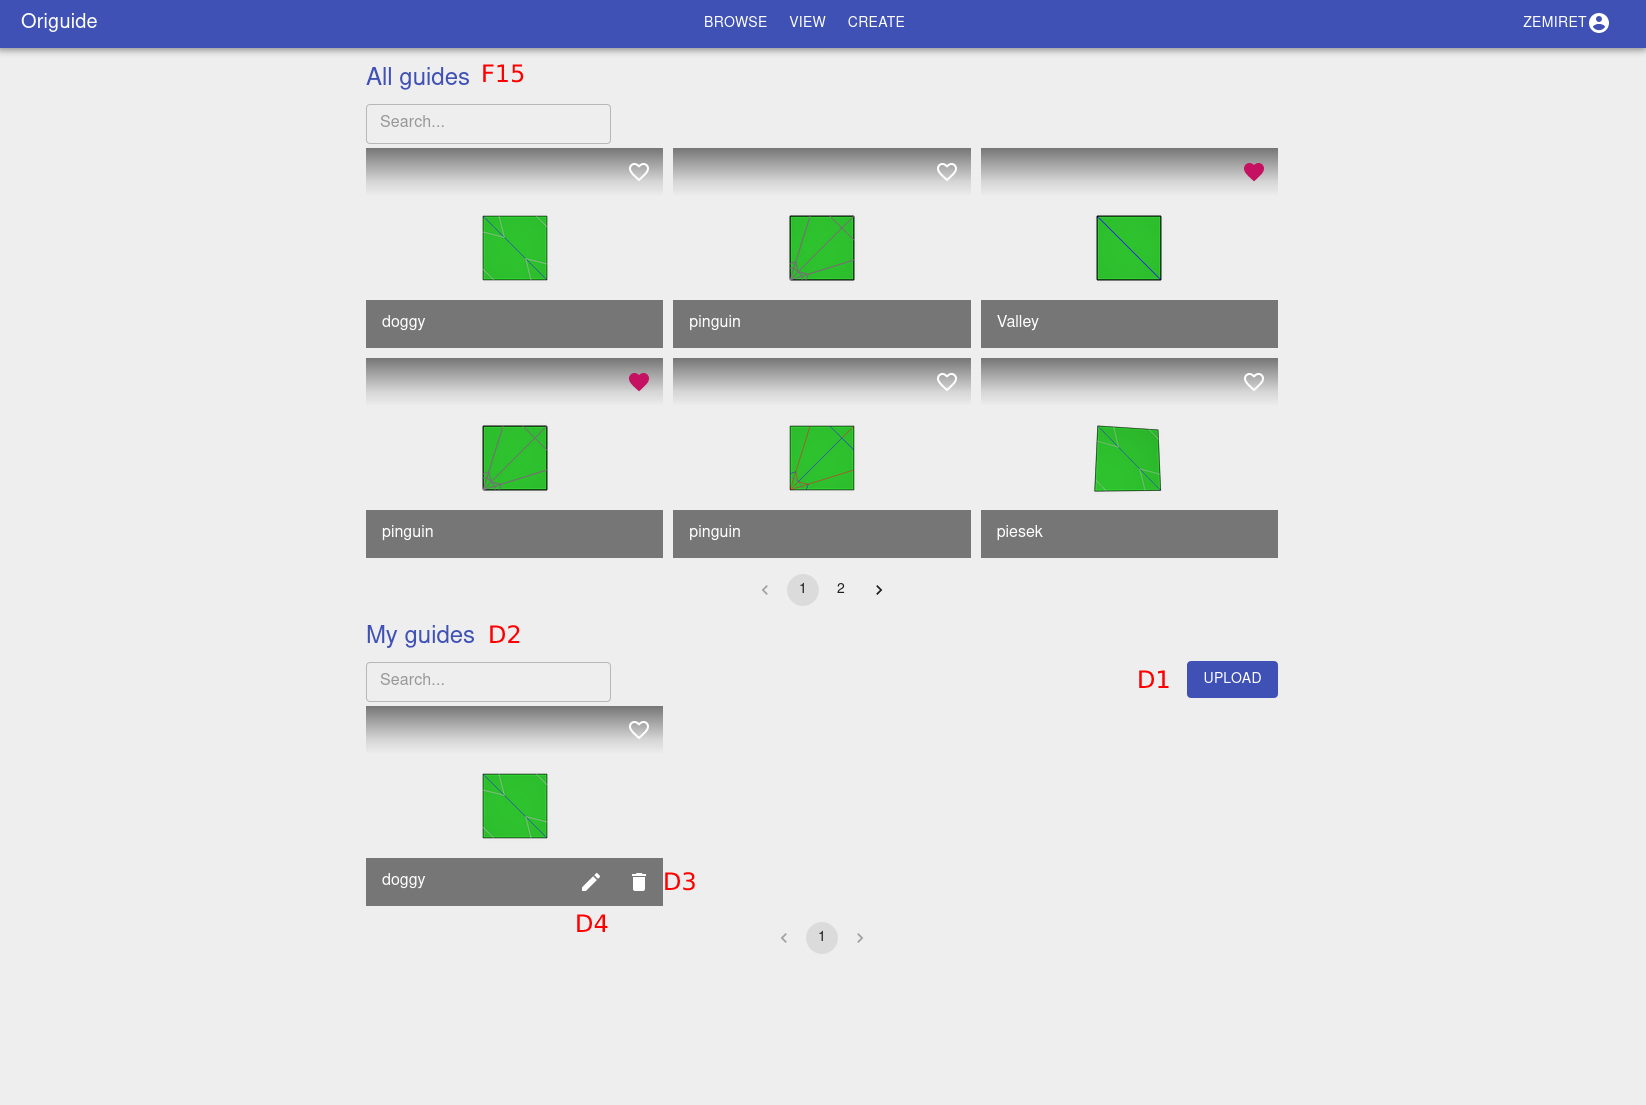
\includegraphics[width=\textwidth]{assets/5-guideBrowser.png}
\end{figure}

\subsubsection{Guide Creator}

Designer's user stories:
\begin{enumerate}
	\setcounter{enumi}{4}
	\requirement{1}{mark my Instructions as public or private}
	\requirement{1}{visually design an Instruction}
	\requirement{1}{save a designed Instruction}
\end{enumerate}

\begin{figure}[H]
  	\centering
    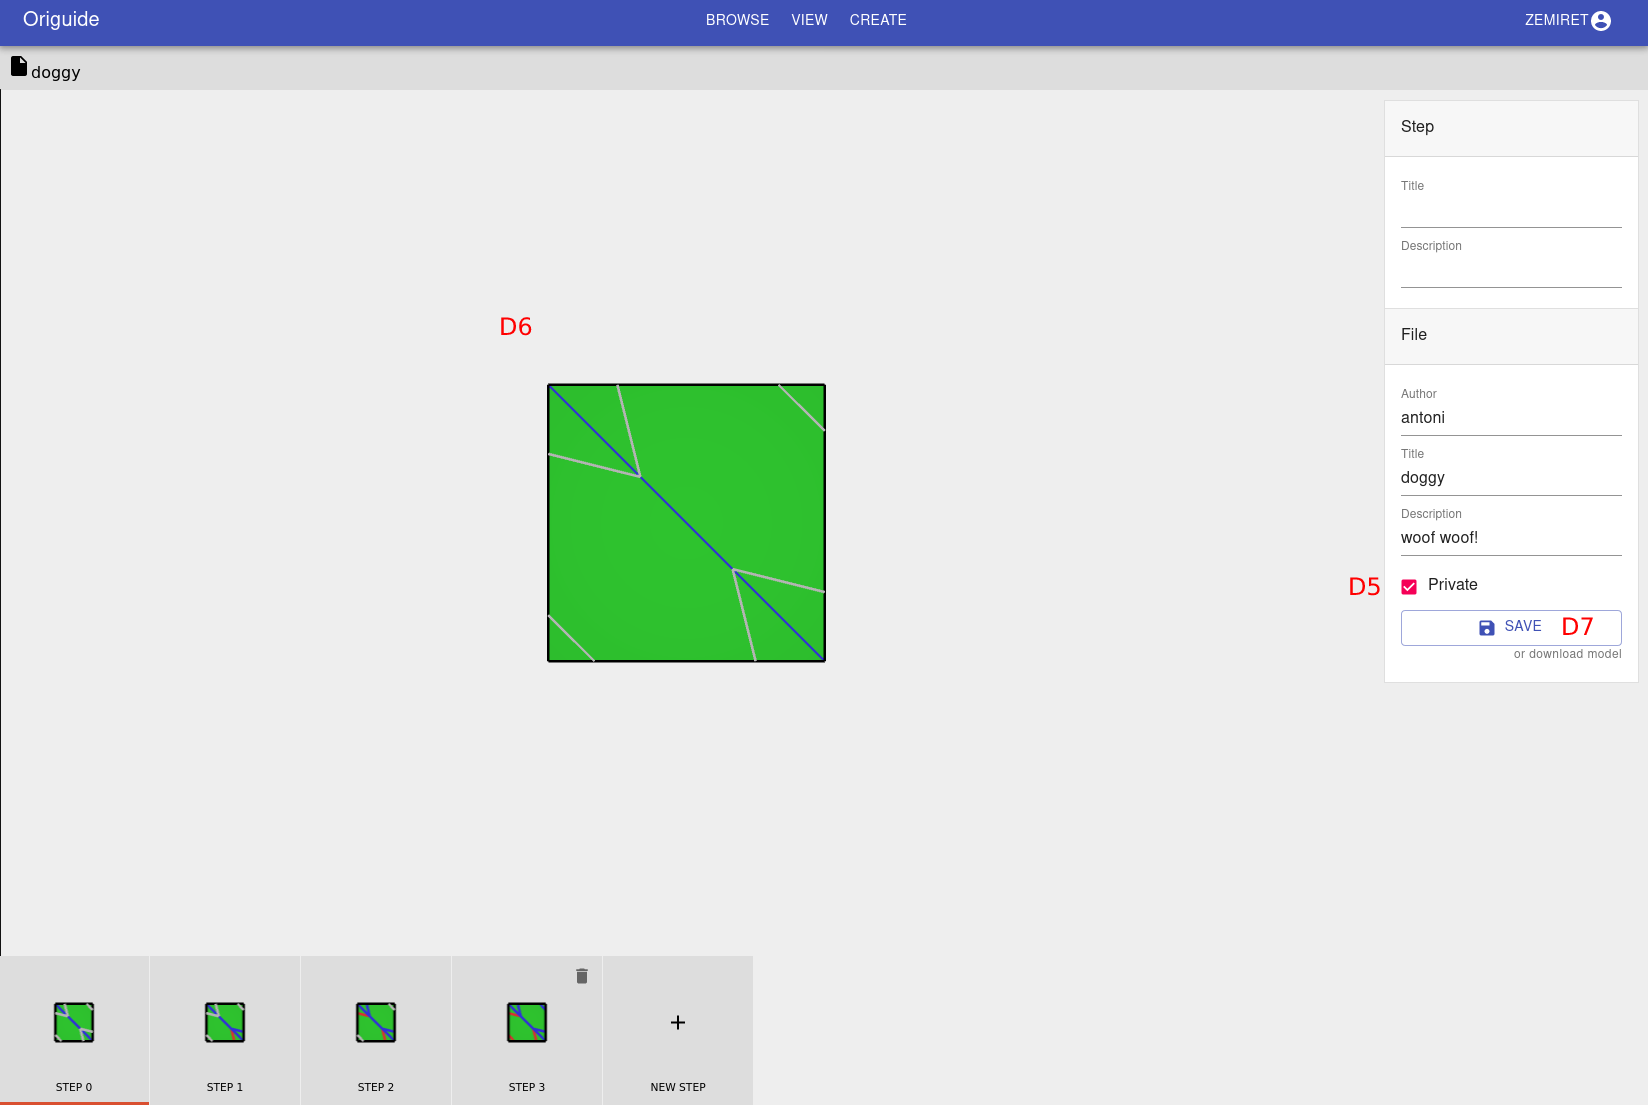
\includegraphics[width=\textwidth]{assets/5-guideCreator.png}
\end{figure}

\subsubsection{Sign up}

Folder's user stories:
\begin{enumerate}
	\setcounter{enumi}{15}
	\requirement{3}{create an account} 
\end{enumerate}

\begin{figure}[H]
  	\centering
    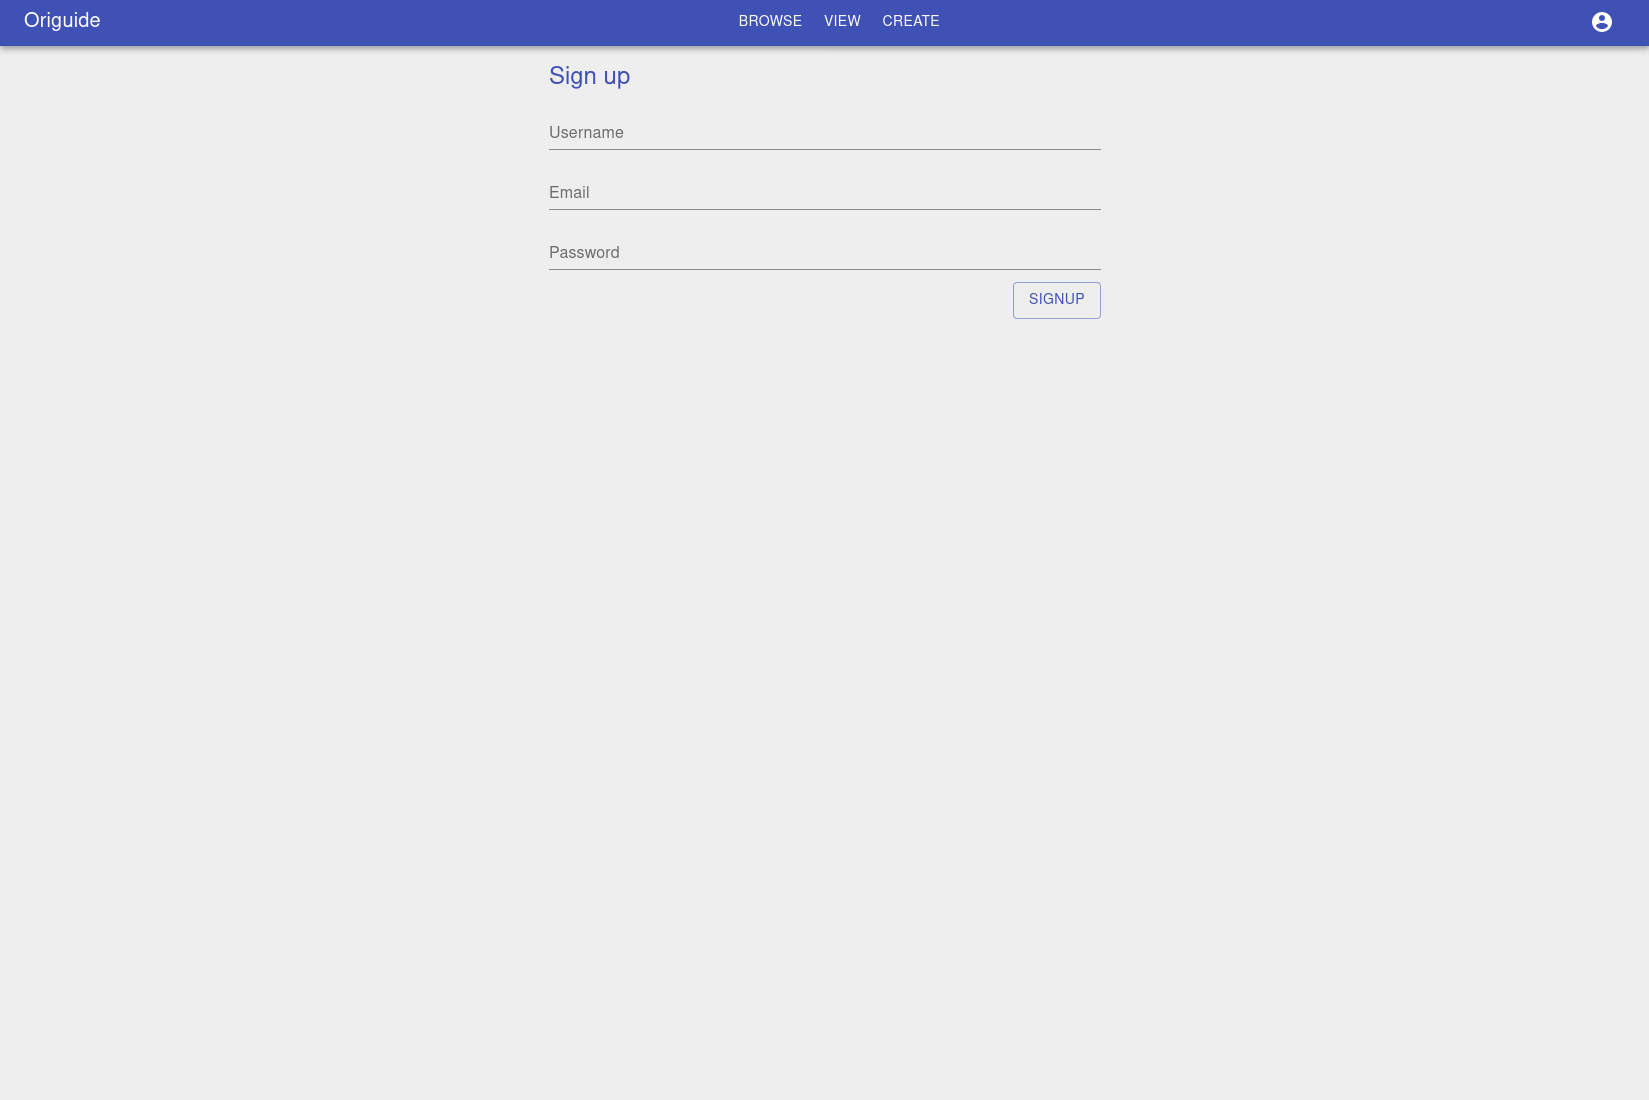
\includegraphics[width=\textwidth]{assets/5-signUp.png}
\end{figure}

\subsubsection{Sign in}

Folder's user stories:
\begin{enumerate}
	\setcounter{enumi}{16}
	\requirement{3}{log into the system} 
\end{enumerate}

\begin{figure}[H]
  	\centering
    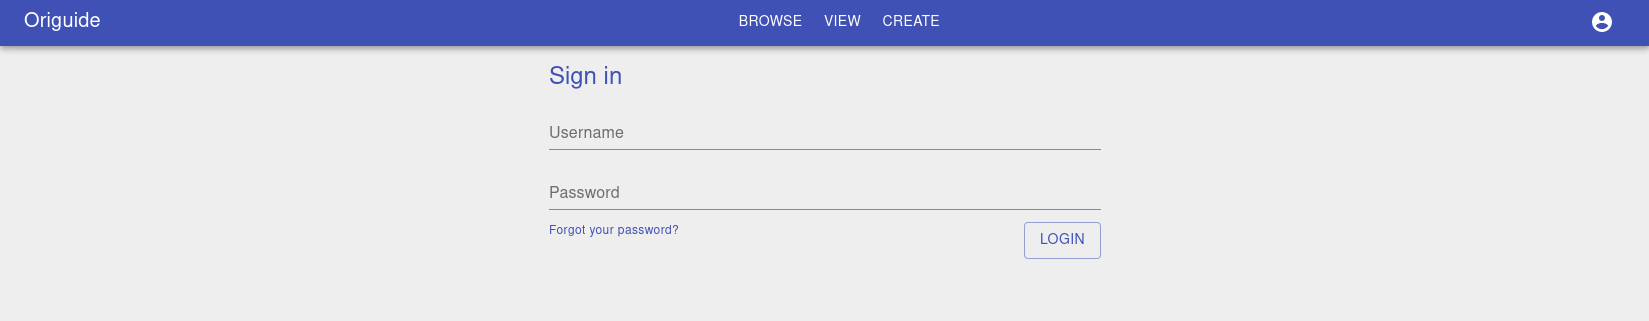
\includegraphics[width=\textwidth]{assets/5-signIn.png}
\end{figure}

\subsubsection{Reset password}

Folder's user stories:
\begin{enumerate}
	\setcounter{enumi}{17}
	\requirement{3}{reset the password} 
\end{enumerate}

\begin{figure}[H]
  	\centering
    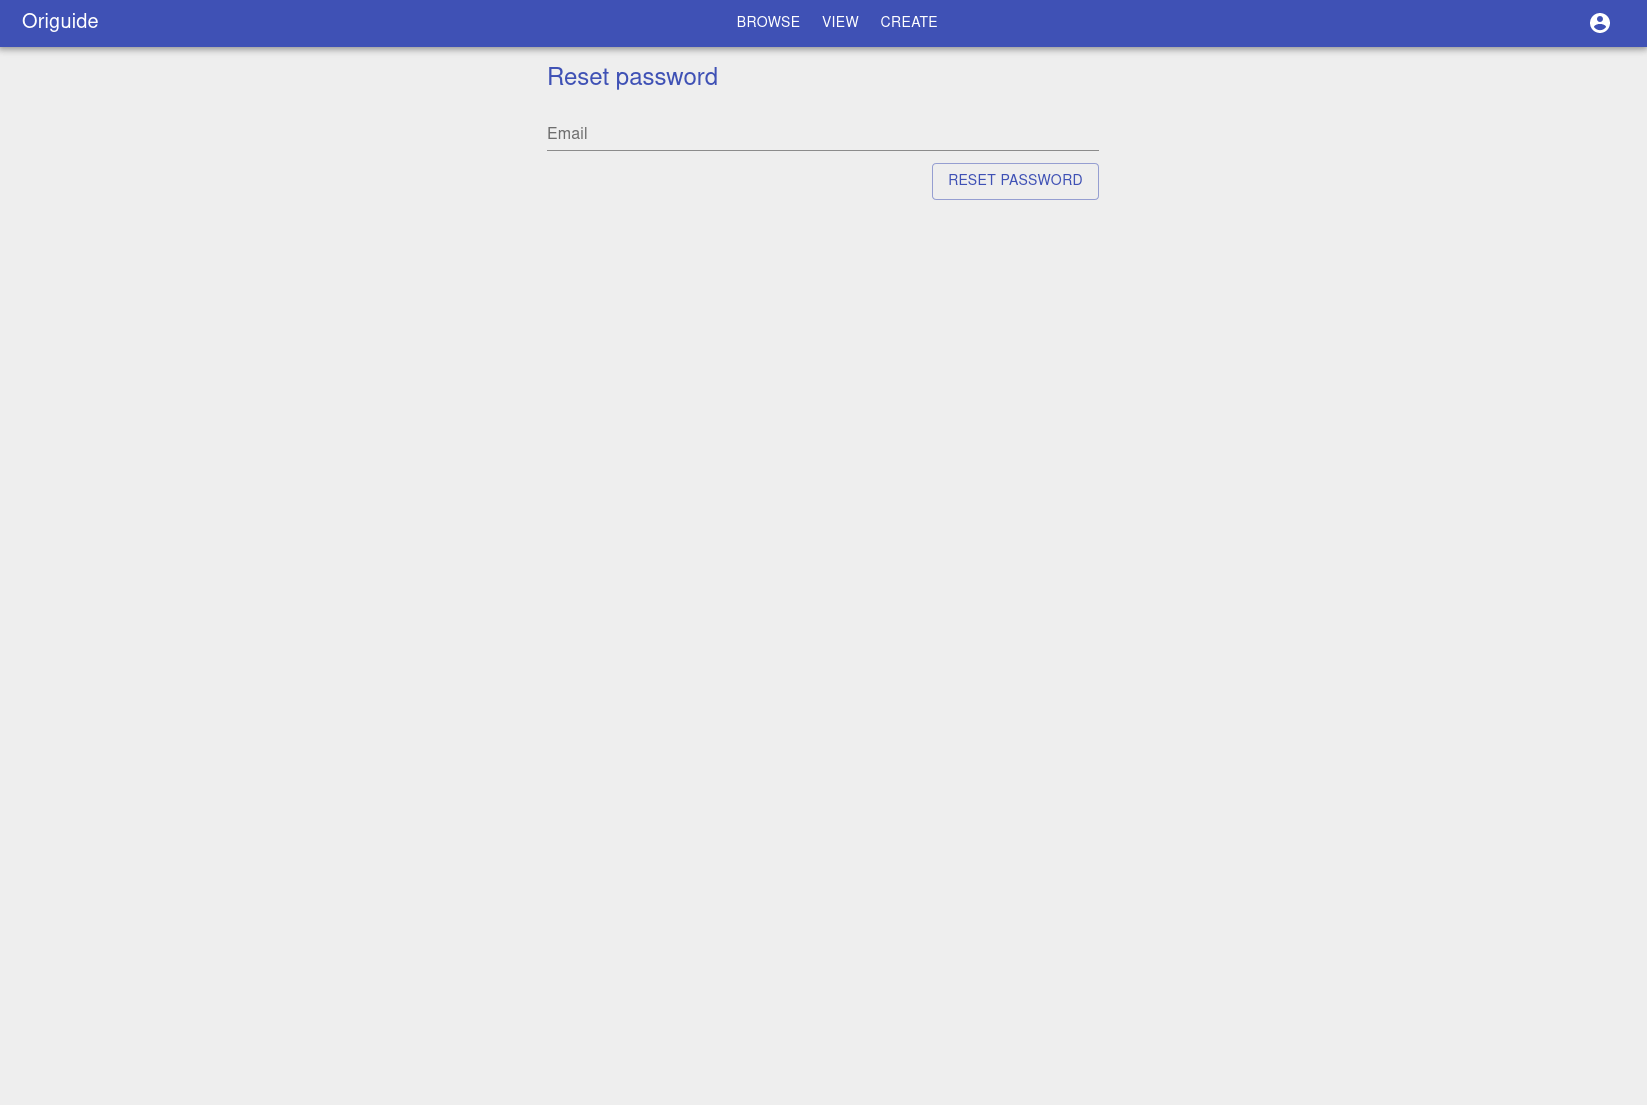
\includegraphics[width=\textwidth]{assets/5-passwordResetForm.png}
\end{figure}

Once the form is submitted, the user receives an email containing password reset instructions.

\begin{figure}[H]
  	\centering
    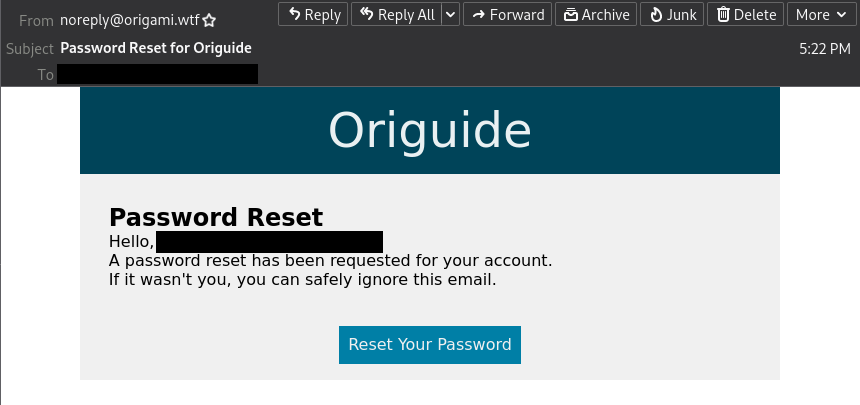
\includegraphics[width=\textwidth]{assets/5-passwordResetEmail.png}
\end{figure}

\subsubsection{Change password}

Folder's user stories:
\begin{enumerate}
	\setcounter{enumi}{18}
	\requirement{2}{change the password} 
\end{enumerate}

\begin{figure}[H]
  	\centering
    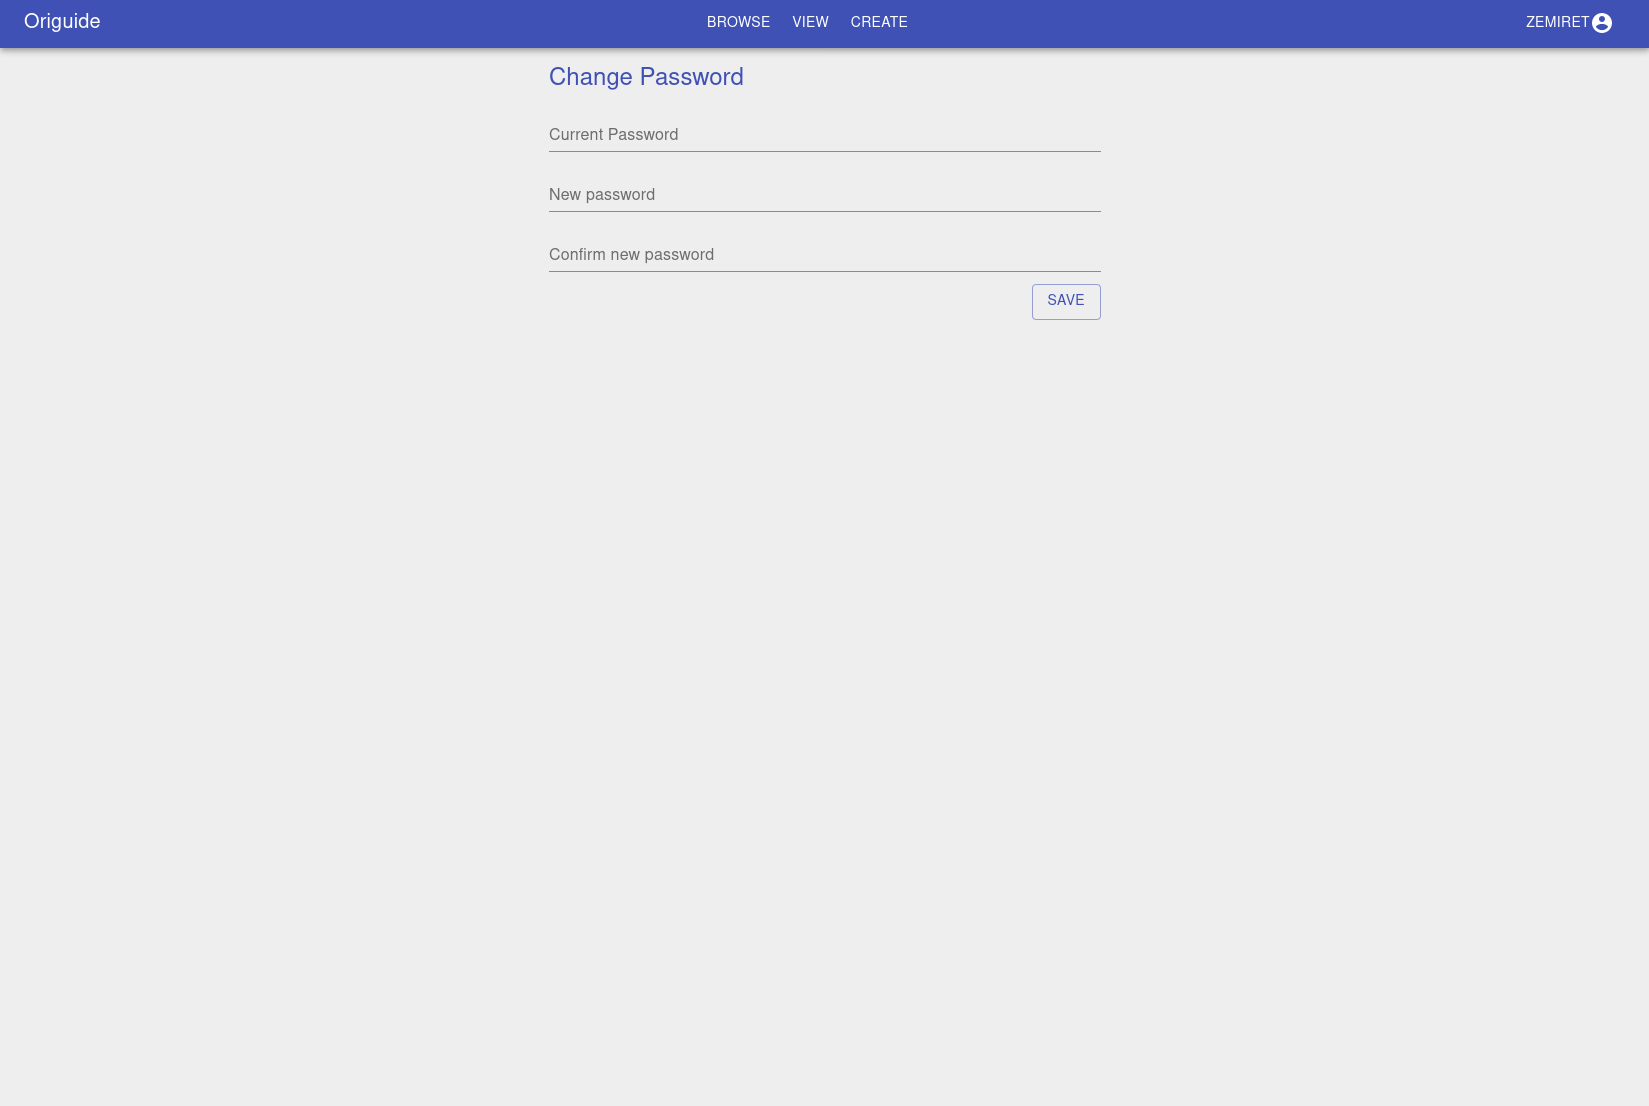
\includegraphics[width=\textwidth]{assets/5-passwordChange.png}
\end{figure}

\subsubsection{Functional requirements that have not been realized}

There are some functional requirements that have not been realized.
All of them happen to be Folder's user stories.
Some proved not to be as important as we had initially assumed.
There are also some that have only been partially accomplished, e.g. they are 
implemented in the backend but no corresponding frontend option is present.
\smallskip

Not realized or partially realized functional requirements:
\begin{enumerate}
	\setcounter{enumi}{12}
	\requirement{1}{change the color of the paper side} 

	
	\setcounter{enumi}{19}
	\requirement{2}{delete the account} 
	\requirement{2}{save another user's Instruction in my account}
	\requirement{1}{mark a saved Instruction as folded} 
\end{enumerate}

\subsubsection{Non-functional requirements}

All but one non-functional requirements have been realized.

The not realized requirement is:
\begin{enumerate}
	\setcounter{enumi}{4}
	\requirement{1}{User should be able to use the application on mobile devices}
\end{enumerate}

Although some parts of our application are usable on mobile devices, 
not everything works as intended. That is not surprising taking into account that
mobile application support had a low priority.


\subsection{Main use cases}
% Prezentacja głównych scenariuszy działania
% Ewentualne skrócone wersje instrukcji (użytkownika, instalacji) - w przypadku kiedy są obszerne proszę je dodać do pracy jako załączniki
% Niekiedy można dodać sekcje FAQ

As defined in the section \nameref{section:project-overview}, there are 2 main 
success paths in the application.
One for Designers and another one for Folders.
These success paths correspond to the main use cases.
In this section we will present these success paths in the context of the end product.

\subsubsection{Designer's success path}

First, the user loads a crease pattern.

\begin{figure}[H]
  	\centering
    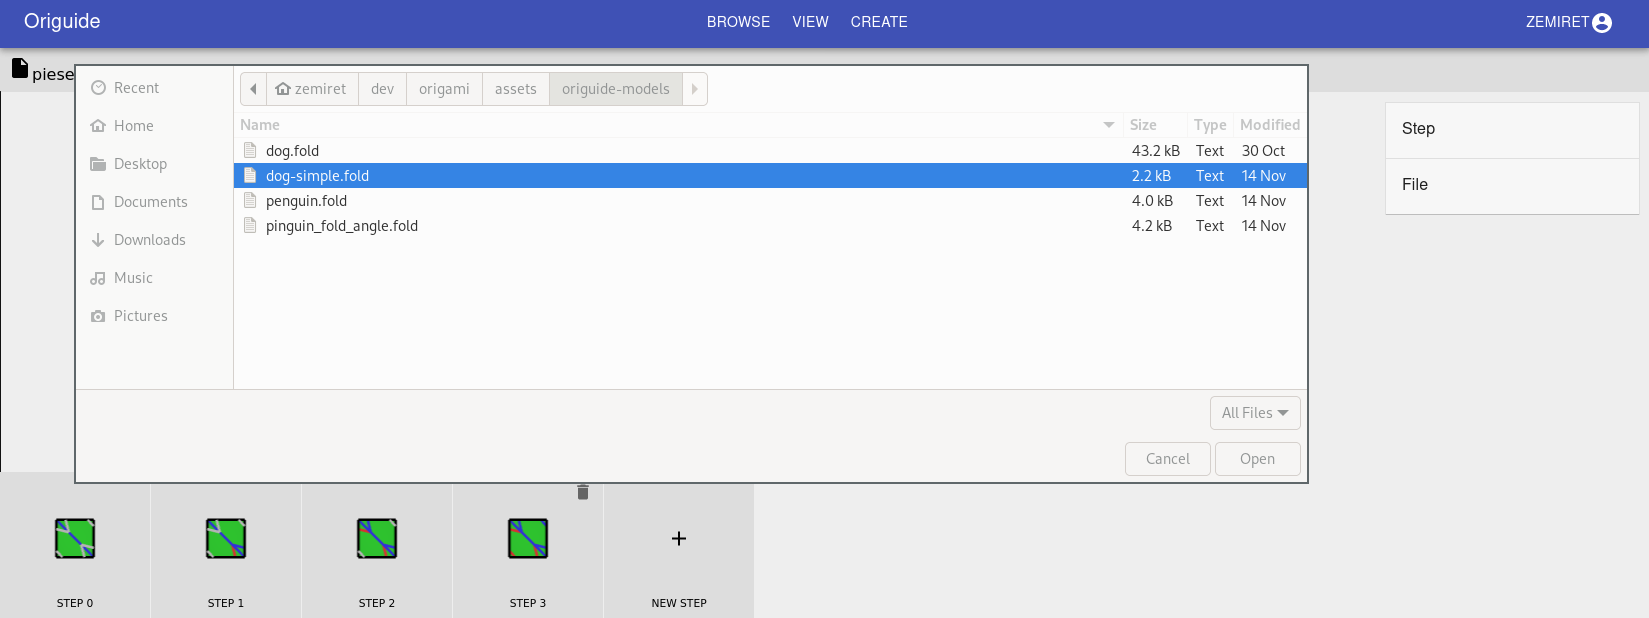
\includegraphics[width=\textwidth]{assets/5-designerLoad.png}
\end{figure}

Next, Guide Creator is shown, and the user proceeds with creating an Instruction.
Once done, the user clicks the \textit{save} button.

\begin{figure}[H]
  	\centering
    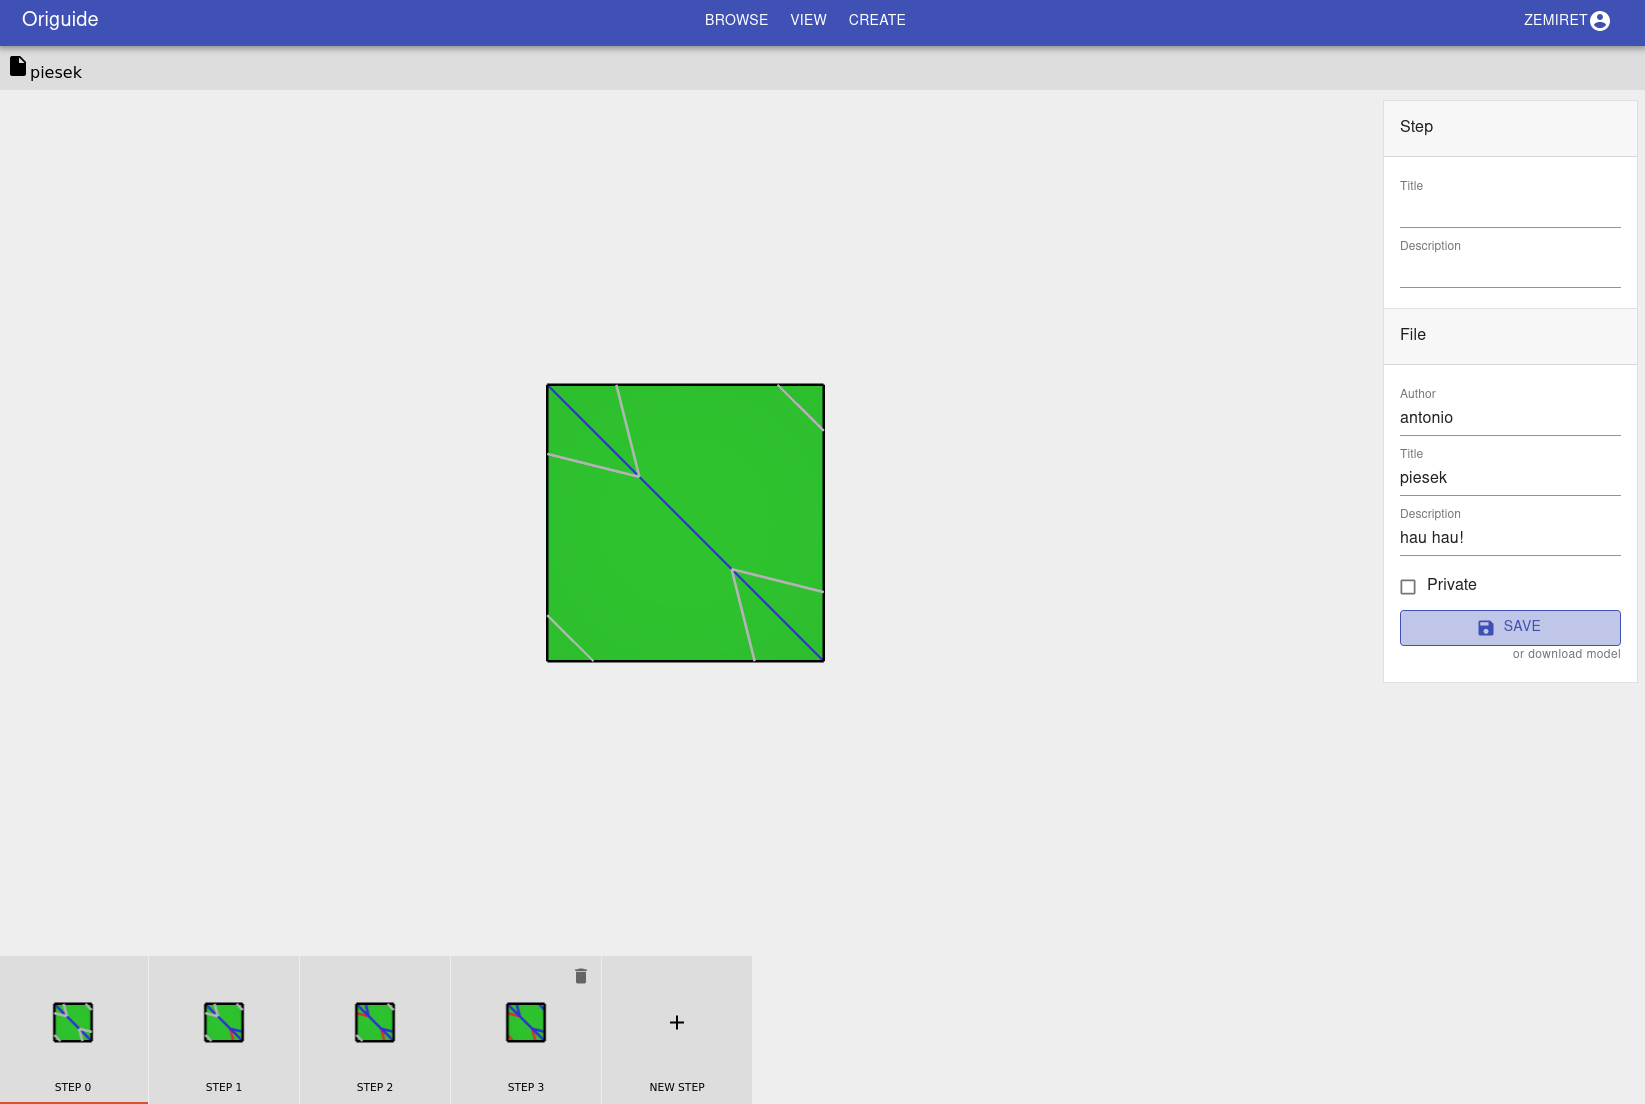
\includegraphics[width=\textwidth]{assets/5-designerSave.png}
\end{figure}

Proper requests are dispatched to the backend, the guide is processed in the background, and
the user is redirected to Guide Browser.

\begin{figure}[H]
  	\centering
    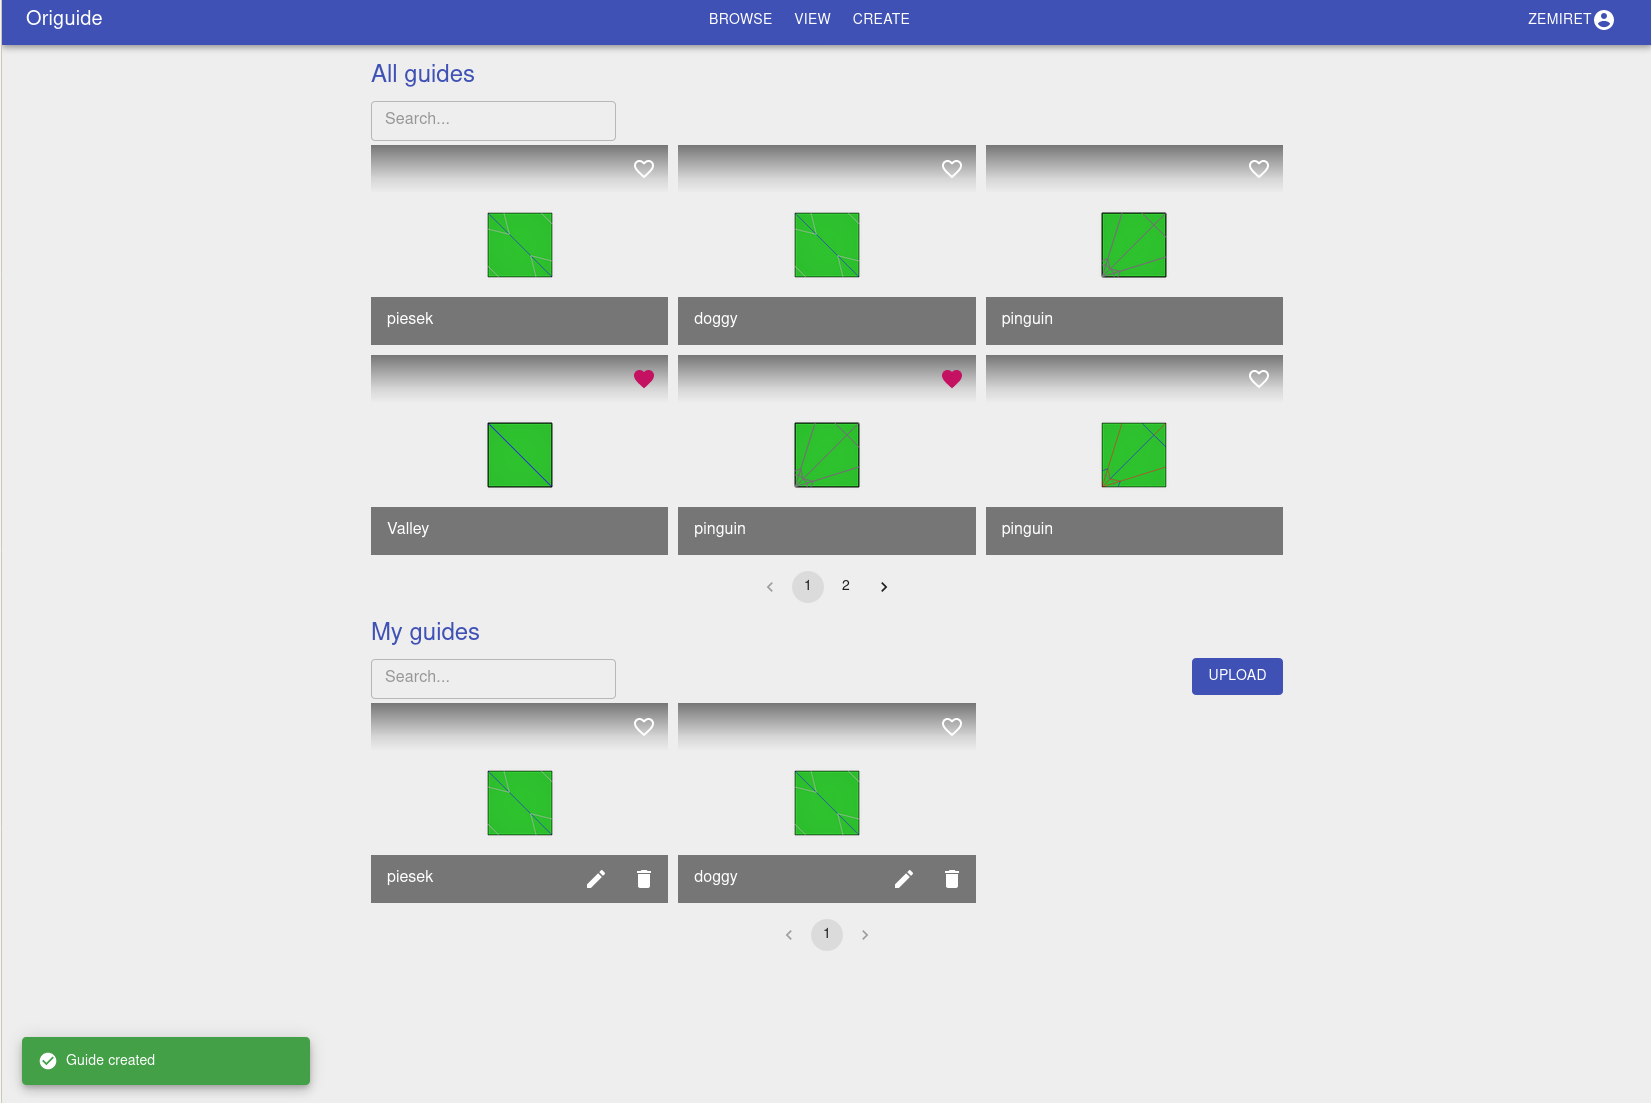
\includegraphics[width=\textwidth]{assets/5-designerBrowser.png}
\end{figure}

\subsubsection{Folder's success path}

The user is presented with Guide Browser. Then, the user clicks on one of the Guides.

\begin{figure}[H]
  	\centering
    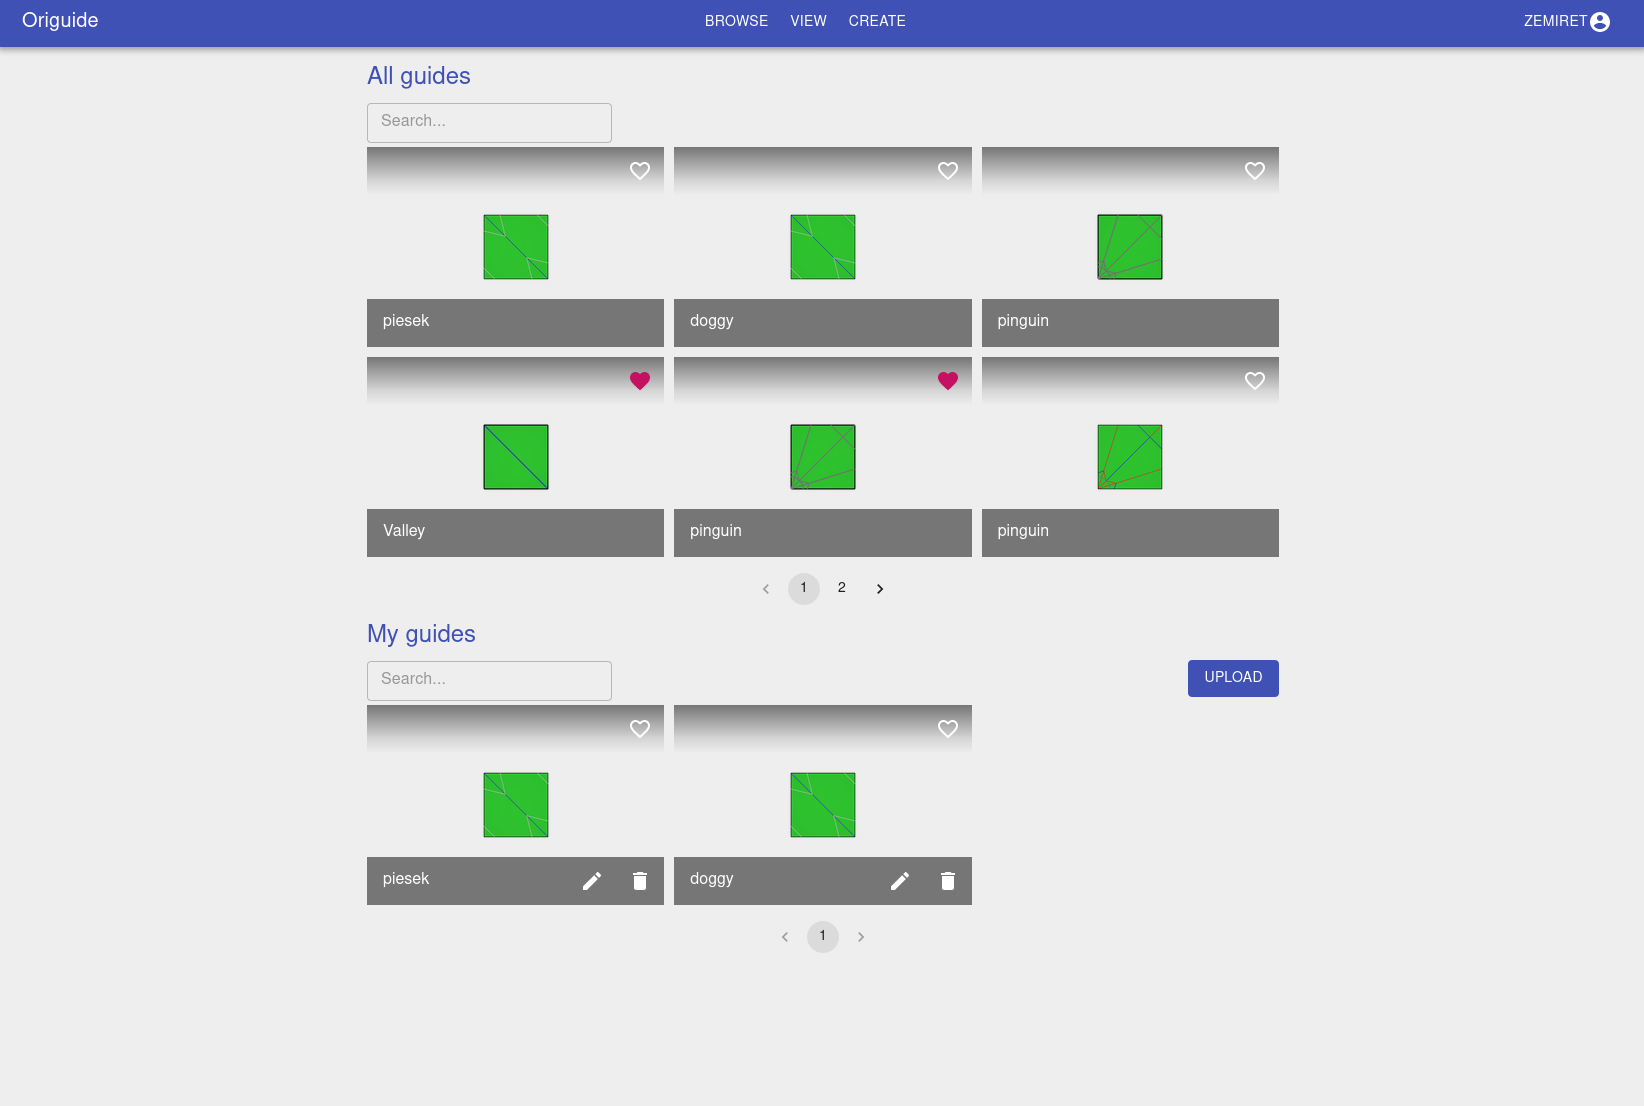
\includegraphics[width=\textwidth]{assets/5-folderOpen.png}
\end{figure}

Once the Guide is loaded, the user is presented with Guide Viewer.

\begin{figure}[H]
  	\centering
    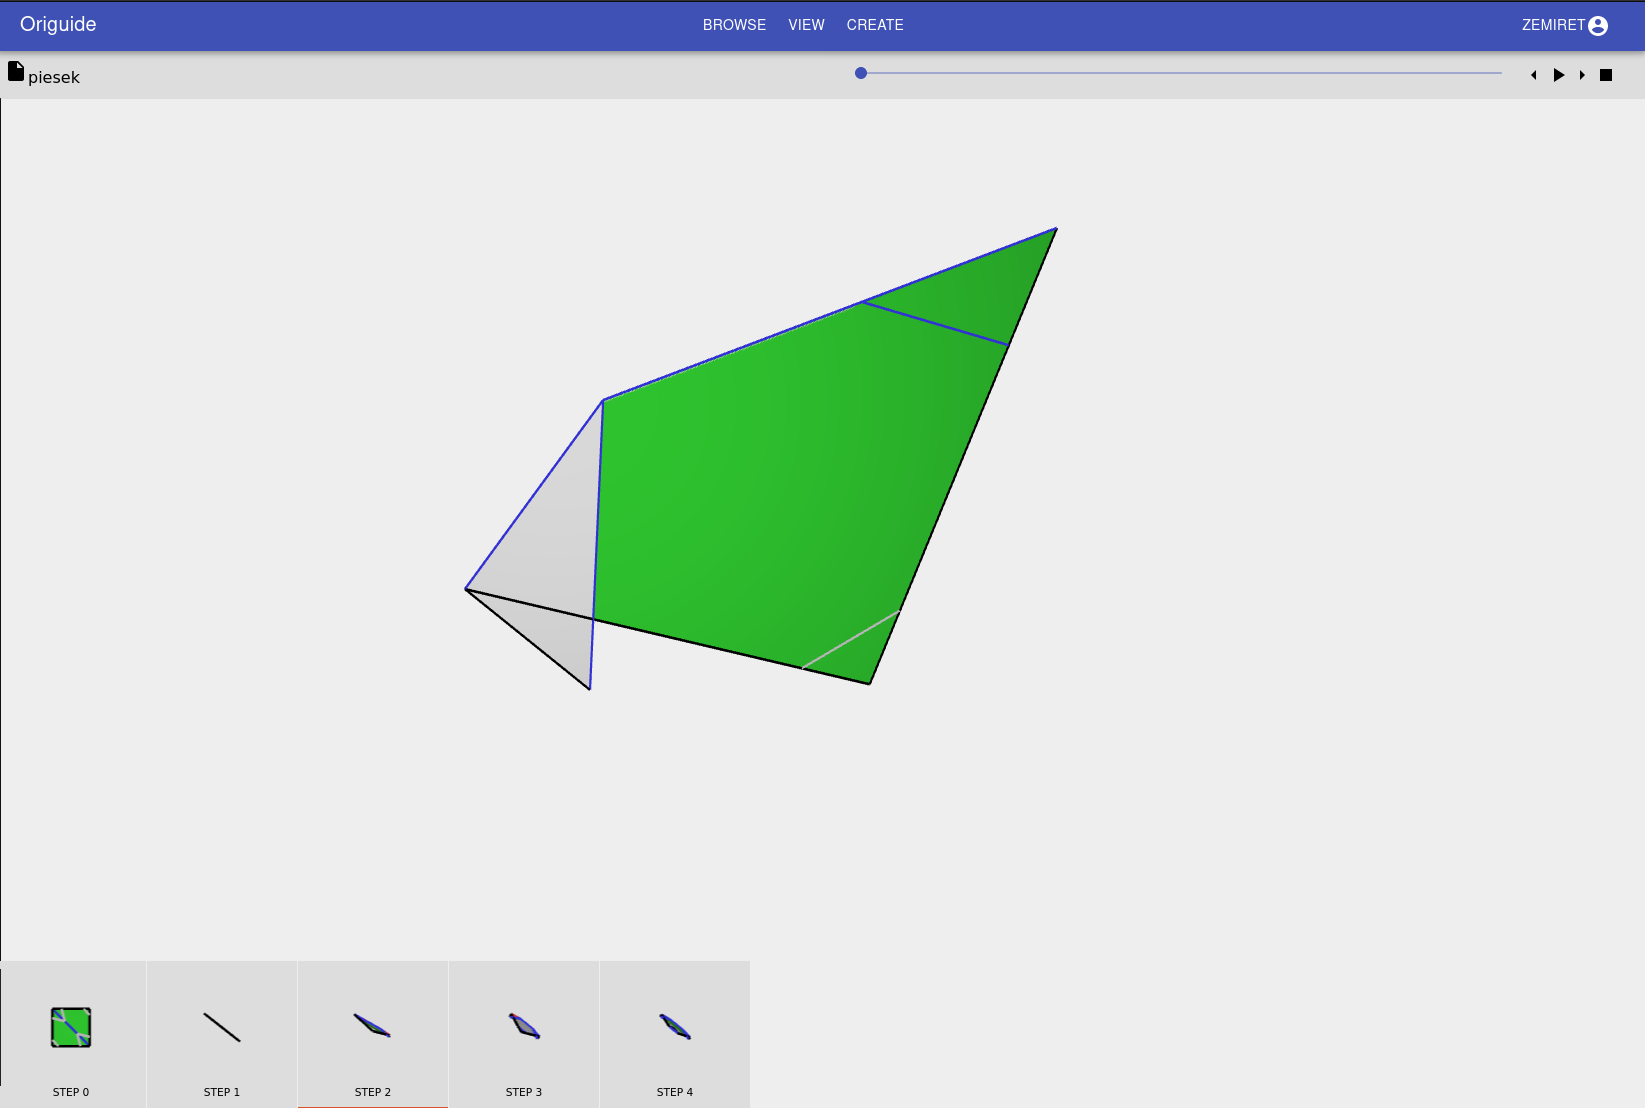
\includegraphics[width=\textwidth]{assets/5-folderView.png}
\end{figure}


\subsection{Project summary}
%Bardzo mile widziane jest podsumowanie wraz z własną subiektywną oceną. Proszę odpowiedzieć sobie i czytelnikowi na pytanie czy projekt się udał, czy jesteście zadowoleni, czy klient jest zadowolony, czego się nauczyliście? Jak można projekt dalej rozwijać?

Overall, we find our project to be a great success.
We have created something interesting both from the scientific and the end user's
point of view. Moreover, our application is something that can be used
by anyone as it is publicly available. Having created the \textit{community}
part of it, we hope to see some real community of origami folders using our product emerge.
\smallskip

Our client seems to be equally happy with the end result.
He appreciates all the work we put into it, 
as well as some more interesting aspects of the project itself.
\smallskip

From the engineering point of view we were confident we can deliver the project.
What at times we found troublesome were some more scientific topics, mostly
connected with how Solver should work.
At some point we were also worried about the performance aspect, but in the end it all worked out well.
During the project we learned a lot about \textit{computational origami} and how to fold a figure or two.
When it comes to the engineering, we did not learn much, but
that is to be expected since we already had some solid foundation in this area.
\smallskip

Although we deem our project complete, it could be developed further as there are a lot of potential areas to work on.
Some of them are:

\begin{itemize}
	\item Collision prevention - although collision detection has been implemented, no prevention is carried out at the moment. At times, this results in some peculiarities during folding.
	\item More sophisticated folding patterns support - right now only figures made out of rigid polygons are supported. In the future, we would like to support some more sophisticated folding patters like inflating or curving.
	\item Improved Guide encoder - folding steps that are produced by Solver are downsampled and encoded to animation frames using some fixed cut-off values. A more robust approach could result in smoother animations.
	\item UI and UX improvements.
	\item Model preview in Guide Creator.
	\item Better thumbnail generation.
\end{itemize}

Even though there is always something more to work on,
both we and our client assumed the current state of the product to be
satisfactory and we are content with the end result.

